\documentclass[border=10pt]{standalone}

\usepackage{tikz}
\usepackage{tikzsymbols}
\usetikzlibrary{calc,patterns,shapes.geometric}

\def\centerarc[#1](#2)(#3:#4:#5){\draw[#1] ($(#2)+({#5*cos(#3)},{#5*sin(#3)})$) arc (#3:#4:#5);}

\begin{document}
	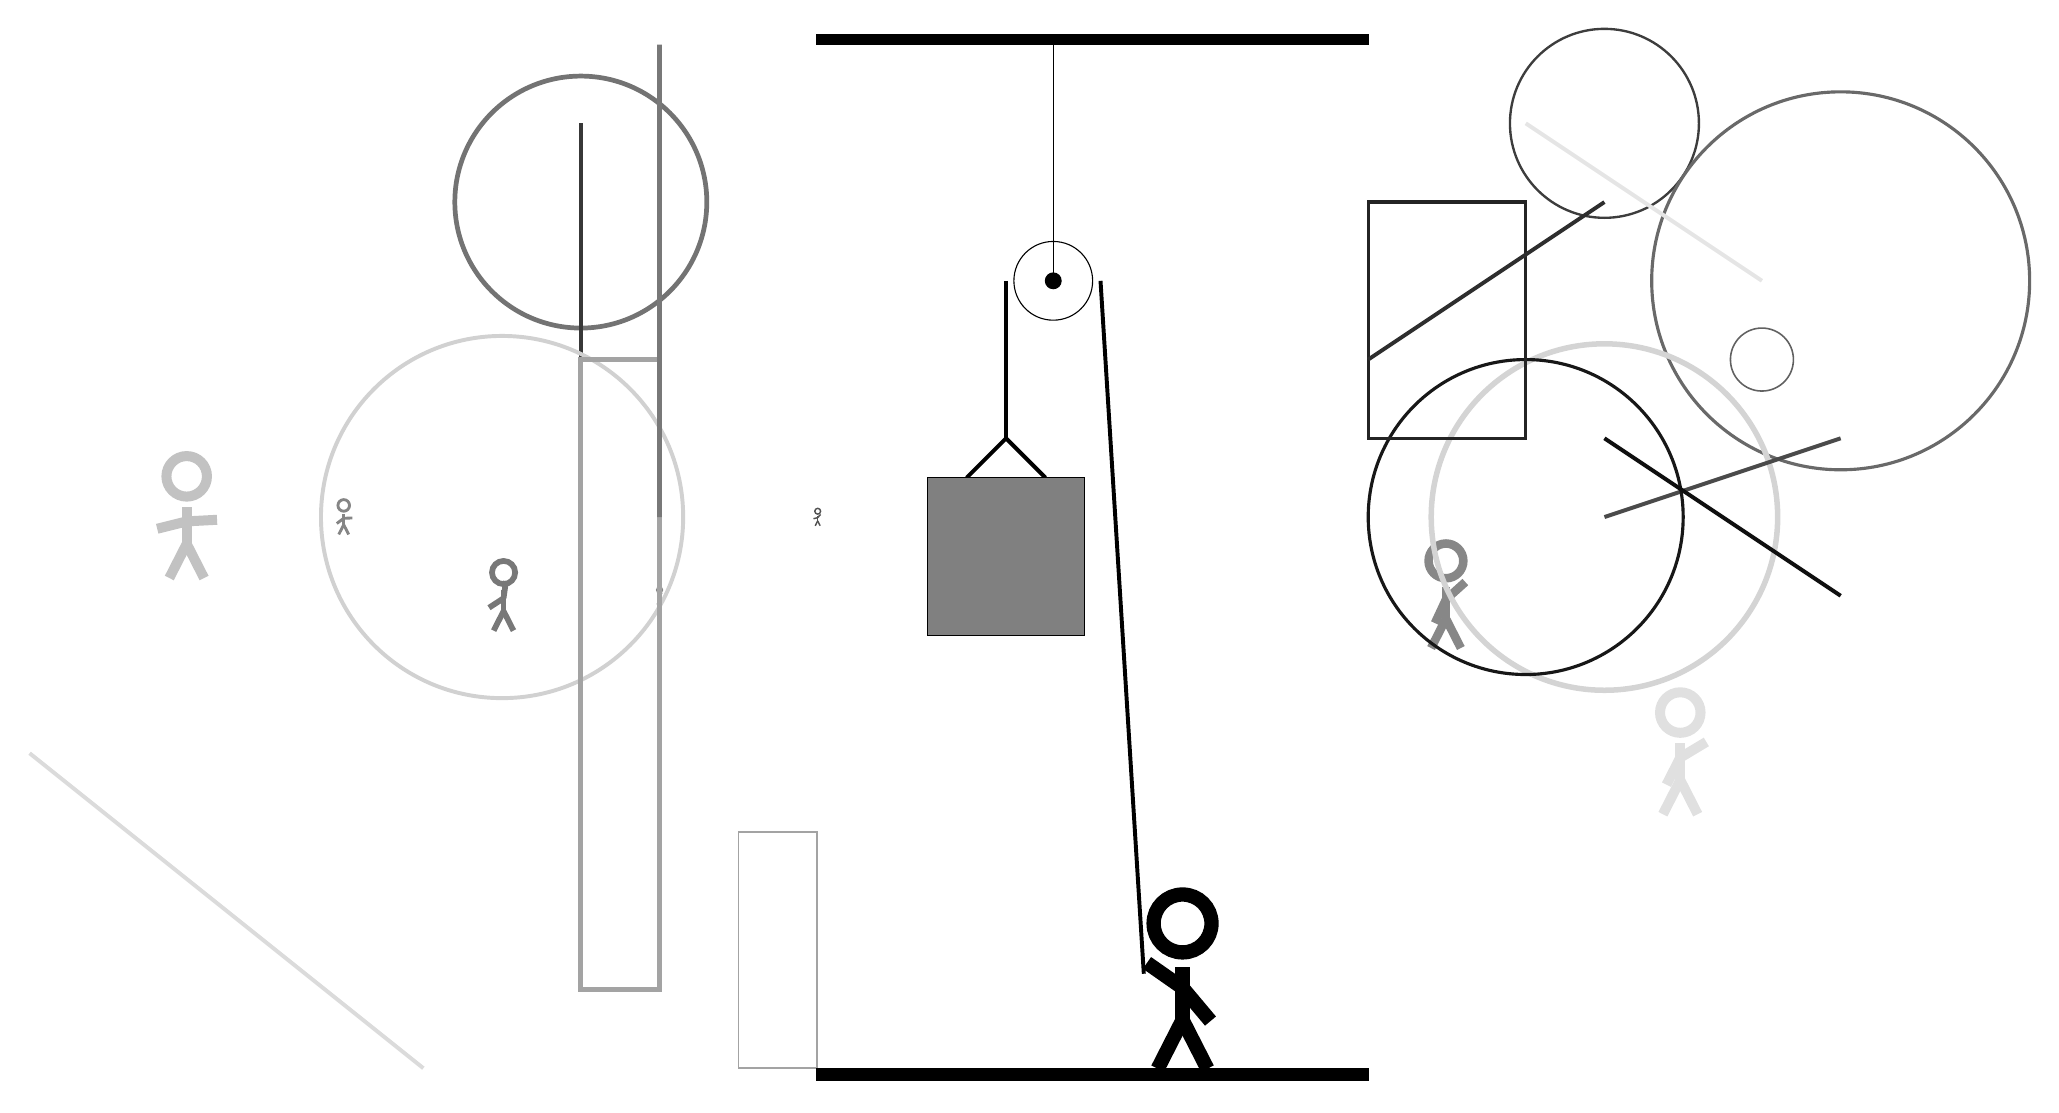
\begin{tikzpicture}
		%%%%% START %%%%%
		
		\draw[fill=black] (-2, 10) rectangle (5, 10.125);
		
		\draw (1, 7) circle (0.5);
		\draw[fill=black] (1, 7) circle (0.1);
		\draw (1, 10) -- (1, 7);
		
		\node[line width=0.2mm, color=black!48] at (-8, 4) {\Strichmaxerl[2][37][2]};
		
		\draw [line width=0.6mm, color=black!55](-5, 8) circle (1.6);
		\node[line width=0.6mm, color=black!24] at (-10, 4) {\Strichmaxerl[7][14][3]};
		\node[line width=0.5mm, color=black!47] at (-4, 3) {\Strichmaxerl[1][88][57]};
		\draw [line width=0.3mm, color=black!76](8, 9) circle (1.2);
		\node[line width=0.6mm, color=black!12] at (9, 1) {\Strichmaxerl[7][63][31]};
		\draw[line width=0.5mm, color=black!14](-7, -3) -- (-12, 1);
		
		\draw[line width=0.5mm, color=black!78](-5, 9) -- (-5, 1);
		\draw [line width=0.4mm, color=black!59](11, 7) circle (2.4);
		\node[line width=0.6mm, color=black!53] at (-6, 3) {\Strichmaxerl[4][33][82]};
		\node[line width=0.3mm, color=black!68] at (-2, 4) {\Strichmaxerl[1][14][48]};
		\node[line width=0.5mm, color=black!47] at (6, 3) {\Strichmaxerl[6][65][42]};
		\draw [line width=0.5mm, color=black!18](-6, 4) circle (2.3);
		
		\draw [line width=0.7mm, color=black!17](8, 4) circle (2.2);
		\draw[line width=0.6mm, color=black!36] (-4, 6) rectangle (-5, -2);
		\draw[line width=0.2mm, color=black!36] (-3, -3) rectangle (-2, 0);
		
		\draw [line width=0.2mm, color=black!62](10, 6) circle (0.4);
		\draw[line width=0.5mm, color=black!71](8, 4) -- (11, 5);
		\draw[line width=0.7mm, color=black!53] (-4, 10) rectangle (-4, 4);
		\draw [line width=0.4mm, color=black!91](7, 4) circle (2.0);
		\draw[line width=0.4mm, color=black!86] (5, 8) rectangle (7, 5);
		
		\draw[line width=0.5mm, color=black!94](8, 5) -- (11, 3);
		\draw[line width=0.5mm, color=black!10](7, 9) -- (10, 7);
		\draw[line width=0.5mm, color=black!82](8, 8) -- (5, 6);
		
		\draw[line width=0.5mm] (-0.1, 4.5) -- (0.4, 5.0) -- (0.9, 4.5);
		\draw[fill=black!50] (-0.6, 4.5) rectangle (1.4, 2.5);
		
		\draw[line width=0.5mm] (0.4, 7) -- (0.4, 5.0);
		\centerarc[line width=0.5mm](1, 7)(0:180:0.6);
		\draw[line width=0.5mm](1.6, 7) -- (2.15, -1.8);
		
		\node at (2.6, -1.9) {\Strichmaxerl[10][-35][-50]};
		
		\draw[fill=black] (-2, -3) rectangle (5, -3.15);
		
		%%%%% END %%%%%
	\end{tikzpicture}
\end{document}